\subsection{Alert Burden and the Deployability Test}
\label{sec:res:alerts}

\emph{Alert volumes.} At the default threshold of 0.5, the transferred detectors raise many false alerts. On the clean flows of \DB{}, their false positive rate is \ROpBCleanFPRmin{} to \ROpBCleanFPRmax, that is, \ROpBCleanAlertsMin{} to \ROpBCleanAlertsMax{} false alerts per hour at our declared rate, for an operational precision of \ROpBCleanPPVmin{} to \ROpBCleanPPVmax{} at $\pi = 0.002$. On all flows, where the copies count as benign, the false positive rate reaches \ROpBAllFPRmax.

\emph{The test.} Table~\ref{tab:test} applies the two-term test of Section~\ref{sec:crit:test}. No detector passes in any label view. On all flows, \RTestAllFailN{} of the six detectors fail and \RTestAllInconclusiveN{} is inconclusive. On the clean flows, the generalization term fails for LR and is inconclusive for the other \RTestCleanGenInconclusiveN{} architectures: their intervals include losses larger than $\delta$, so neither a pass nor a failure is established. The alert term fails for \RTestCleanAlertFailN{} architectures and is inconclusive for \RTestCleanAlertInconclusiveN{}. Its intervals are wide because the threshold fixed on the source data of each split lands differently on the target: across the 20 splits, one architecture can range from no alerts, and no detections, to tens of thousands of false alerts per hour. Counted split by split, HGB meets all three alert conditions in \RJointHGBClean{} of the 20 splits, the MLP in \RJointMLPClean{}, XGB in \RJointXGBClean{}, and the other architectures in none. Averaged over the splits, HGB raises \RTestHGBCleanAlerts{} false alerts per hour at a recall of \RTestHGBCleanRecall{} and an operational precision of \RTestHGBCleanPPV{}, more alerts than our bound allows. Relabeling the copies gives the same verdicts except for RF, whose alert term becomes inconclusive.

\begin{table*}[t]
\caption{Two-term deployability test (Section~\ref{sec:crit:test}) for transfer from \DA{} to \DB{}, 20 splits. Generalization: $\Delta_{\mathrm{BA}}$ with its Nadeau--Bengio corrected 95\% interval; pass if the upper bound is at most $\delta = 0.10$, fail if the lower bound exceeds it. Alert burden at the threshold fixed on each split's held-out source data (recall at least 0.5 there): mean recall, false alerts per hour at $\lambda_b = 240{,}000$ benign flows per hour, and operational precision at $\pi = 0.002$, with corrected intervals; pass if all three intervals lie on the passing side of $r_{\min} = 0.5$, $A_{\max} = 200$, and $\rho = 0.1$, fail if any lies on the failing side. Splits: splits in which all three alert conditions hold. $\checkmark$: pass, $\times$: fail, ?: inconclusive; $\mathcal{P}$: verdict. The bounds are our own, not operator requirements.}
\label{tab:test}
\centering
\scriptsize
\setlength{\tabcolsep}{3pt}
\begin{tabular}{llcccccccc}
\toprule
 & & \multicolumn{2}{c}{Generalization} & \multicolumn{5}{c}{Alert burden, threshold fixed on source data} & \\
\cmidrule(lr){3-4}\cmidrule(lr){5-9}
View & Model & $\Delta_{\mathrm{BA}}$ [95\% CI] & & Recall [95\% CI] & Alerts/h [95\% CI] & PPV [95\% CI] & Splits & & $\mathcal{P}$ \\
\midrule
All flows & LR & +0.21 [0.10, 0.31] & ? & 0.04 [0.00, 0.09] & 570 [0, 1{,}832] & 0.032 [0.000, 1.000] & 0/20 & $\times$ & $\times$ \\
 & DT & +0.25 [0.06, 0.45] & ? & 0.70 [0.41, 0.98] & 146{,}512 [88{,}607, 204{,}416] & 0.002 [0.001, 0.005] & 0/20 & $\times$ & $\times$ \\
 & RF & +0.22 [$-$0.02, 0.46] & ? & 0.14 [0.00, 0.47] & 31{,}967 [0, 107{,}201] & 0.002 [0.000, 1.000] & 0/20 & $\times$ & $\times$ \\
 & XGB & +0.28 [0.07, 0.48] & ? & 0.19 [0.00, 0.58] & 45{,}441 [0, 137{,}454] & 0.002 [0.000, 1.000] & 0/20 & ? & ? \\
 & HGB & +0.28 [0.10, 0.47] & ? & 0.51 [0.16, 0.86] & 113{,}355 [38{,}968, 187{,}742] & 0.002 [0.000, 0.011] & 0/20 & $\times$ & $\times$ \\
 & MLP & +0.38 [0.22, 0.55] & $\times$ & 0.39 [0.00, 0.84] & 85{,}583 [0, 189{,}405] & 0.002 [0.000, 1.000] & 0/20 & ? & $\times$ \\
\midrule
Clean & LR & +0.22 [0.11, 0.33] & $\times$ & 0.04 [0.00, 0.09] & 1{,}387 [0, 4{,}460] & 0.014 [0.000, 1.000] & 0/20 & $\times$ & $\times$ \\
 & DT & +0.04 [$-$0.17, 0.25] & ? & 0.70 [0.41, 0.98] & 46{,}906 [0, 127{,}390] & 0.007 [0.002, 1.000] & 0/20 & ? & ? \\
 & RF & $-$0.01 [$-$0.27, 0.25] & ? & 0.14 [0.00, 0.47] & 101 [0, 511] & 0.406 [0.000, 1.000] & 0/20 & $\times$ & $\times$ \\
 & XGB & +0.01 [$-$0.23, 0.24] & ? & 0.19 [0.00, 0.58] & 41 [0, 259] & 0.691 [0.000, 1.000] & 2/20 & ? & ? \\
 & HGB & +0.01 [$-$0.19, 0.20] & ? & 0.51 [0.16, 0.86] & 352 [0, 2{,}845] & 0.412 [0.027, 1.000] & 12/20 & ? & ? \\
 & MLP & +0.21 [$-$0.05, 0.48] & ? & 0.39 [0.00, 0.84] & 1{,}762 [0, 7{,}043] & 0.096 [0.000, 1.000] & 4/20 & ? & ? \\
\midrule
Relabeled & LR & +0.26 [0.15, 0.37] & $\times$ & 0.03 [0.00, 0.06] & 1{,}387 [0, 4{,}460] & 0.010 [0.000, 1.000] & 0/20 & $\times$ & $\times$ \\
 & DT & +0.02 [$-$0.20, 0.24] & ? & 0.75 [0.45, 1.00] & 46{,}906 [0, 127{,}390] & 0.008 [0.002, 1.000] & 0/20 & ? & ? \\
 & RF & $-$0.03 [$-$0.29, 0.23] & ? & 0.17 [0.00, 0.55] & 101 [0, 511] & 0.442 [0.000, 1.000] & 0/20 & ? & ? \\
 & XGB & $-$0.02 [$-$0.26, 0.22] & ? & 0.23 [0.00, 0.69] & 41 [0, 259] & 0.728 [0.000, 1.000] & 2/20 & ? & ? \\
 & HGB & $-$0.02 [$-$0.22, 0.17] & ? & 0.59 [0.20, 0.99] & 352 [0, 2{,}845] & 0.448 [0.032, 1.000] & 12/20 & ? & ? \\
 & MLP & +0.19 [$-$0.08, 0.46] & ? & 0.45 [0.00, 0.98] & 1{,}762 [0, 7{,}043] & 0.109 [0.000, 1.000] & 4/20 & ? & ? \\
\bottomrule
\end{tabular}

\end{table*}

\emph{An optimistic bound.} A threshold searched on the target shows what the ranking itself allows. With the best such threshold, HGB reaches an operational precision of \ROracleHGBCleanPPV{} at \ROracleHGBCleanAlerts{} false alerts per hour on the clean flows, and XGB \ROracleXGBCleanPPV{} at \ROracleXGBCleanAlerts{}, both within our bounds; \RTestCleanOracleN{} architectures meet the bounds in this way, and none does on all flows, where the best operational precision at a recall of at least 0.5 is \RTestAllOraclePPVmax. On consistent labels the best transferred detectors therefore rank the attacks of \DB{} well enough for our bounds, but the threshold that would realize this cannot be chosen from source data. In our experiments the threshold, not only the model, had to be set with labeled data from the target.

\begin{figure*}[t]
\centering
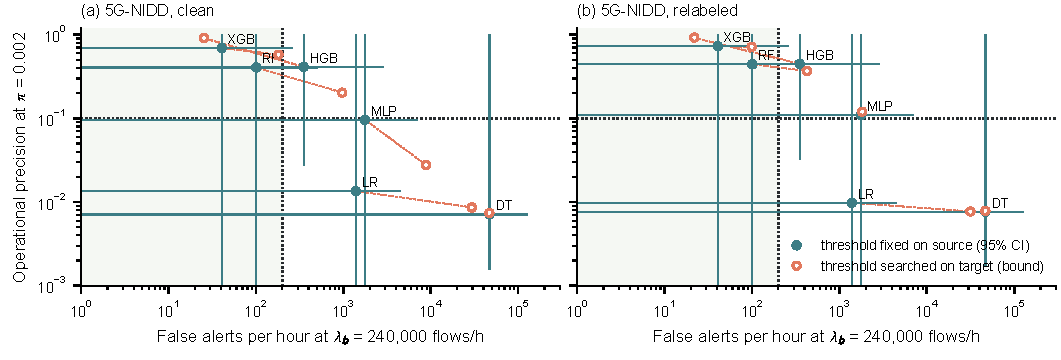
\includegraphics[width=0.92\textwidth]{figs/fig_test}
\caption{Where the transferred detectors lie relative to the alert bounds on \DB{}: false alerts per hour against operational precision, mean over 20 splits, at the threshold fixed on source data (filled, with corrected 95\% intervals) and at the best threshold searched on the target (open, an optimistic bound), for (a) clean flows and (b) copies relabeled. The shaded region meets $A_{\max} = 200$ false alerts per hour; dotted lines mark $A_{\max}$ and $\rho = 0.1$. Both bounds are our own choices; another operator would move the lines.}
\label{fig:test}
\end{figure*}

\emph{Sensitivity to the bounds.} The bounds are our own, and Fig.~\ref{fig:test} shows how far each detector lies from them. On all flows no threshold comes close: even the threshold searched on the target leaves every architecture with at least \RTestAllOracleAlertsMin{} false alerts per hour at a recall of 0.5. On consistent labels the verdict depends on the threshold rule more than on the bounds. At the threshold fixed on source data, the recall interval of every architecture extends below $r_{\min} = 0.5$, so no change of $A_{\max}$ or $\rho$ alone would make the alert term pass, and the generalization term would remain inconclusive unless $\delta$ were raised to \RTestCleanGenHiMin, the smallest upper bound of $\Delta_{\mathrm{BA}}$ on these flows.
